\documentclass{article}
\usepackage{graphicx} % Required for inserting images
\usepackage[utf8]{inputenc}
\usepackage{hyperref}
\usepackage[letterpaper, portrait, margin=1in]{geometry}
\usepackage{enumitem}
\usepackage{amsmath}
\usepackage{booktabs}
\usepackage{graphicx}
\usepackage{float}
\usepackage{hyperref}
\usepackage[flushleft]{threeparttable}
\usepackage{textcomp}
\hypersetup
{
colorlinks=true,
    linkcolor=black,
    filecolor=black,      
    urlcolor=blue,
    citecolor=black,
}




\usepackage{titlesec}
  
\title{Homework 6 Submission}
\author{David Wilson \\ Economics 7103}

  
\begin{document}
  
\maketitle

\section{Hourly data - Stata}

\begin{enumerate}
\setcounter{enumi}{1}
\item The number of ATTs with negative weights is 48,547.


\item I clustered at the individual level. The estimates are below in Table 1.

\begin{table}[H]
    \centering
    \caption{Two-Way Fixed Effects Estimates at the Hourly Level}
    \begin{threepart}
        {
\def\sym#1{\ifmmode^{#1}\else\(^{#1}\)\fi}
\begin{tabular}{l*{1}{c}}
\hline\hline
                    &\multicolumn{1}{c}{Energy Consumption (kWh)}\\
\hline
ATT                 &     -0.0434\sym{***}\\
                    &    (0.0002)         \\
[1em]
Temperature (F)     &      0.0046\sym{***}\\
                    &    (0.0000)         \\
[1em]
Precipitation (in)  &     -0.0006         \\
                    &    (0.0020)         \\
[1em]
Relative Humidity (\%)&      0.0023\sym{***}\\
                    &    (0.0000)         \\
[1em]
Constant            &      0.5387\sym{***}\\
                    &    (0.0011)         \\
\hline
Observations        &      720000         \\
Adjusted \(R^{2}\)  &       0.663         \\
\hline\hline
\multicolumn{2}{l}{\footnotesize Standard errors in parentheses}\\
\multicolumn{2}{l}{\footnotesize \sym{*} \(p<0.05\), \sym{**} \(p<0.01\), \sym{***} \(p<0.001\)}\\
\end{tabular}
}

    \end{threepart}
\end{table}
\end{enumerate}
\section{Daily data - Stata}

\begin{enumerate}

\item At first glance they differ a lot, but then when we take into consideration that the first question is at the hourly level. When scaled up to the daily level, they are similar. The R$^2$ is about a third lower at the daily level.

\begin{table}[H]
    \centering
    \caption{Two-Way Fixed Effects Estimates at the Daily Level}
    \begin{threepart}
        {
\def\sym#1{\ifmmode^{#1}\else\(^{#1}\)\fi}
\begin{tabular}{l*{1}{c}}
\hline\hline
                    &\multicolumn{1}{c}{Energy usage (kWh)}\\
\hline
ATT                 &     -0.9356\sym{***}\\
                    &    (0.0056)         \\
[1em]
Temperature (F)     &      0.1109\sym{***}\\
                    &    (0.0004)         \\
[1em]
Precipitation (inches)&      0.0681         \\
                    &    (0.1882)         \\
[1em]
Relative Humidity (\%)&      0.0552\sym{***}\\
                    &    (0.0002)         \\
[1em]
Constant            &     12.8783\sym{***}\\
                    &    (0.0341)         \\
\hline
Observations        &       30000         \\
Adjusted \(R^{2}\)  &       0.971         \\
\hline\hline
\multicolumn{2}{l}{\footnotesize Standard errors in parentheses}\\
\multicolumn{2}{l}{\footnotesize \sym{*} \(p<0.10\), \sym{**} \(p<0.05\), \sym{***} \(p<0.01\)}\\
\end{tabular}
}

    \end{threepart}
\end{table}

\item Figure 1 contains the event-study using reghdfe and plotted using coefplot. 
\begin{figure}[H]
    \centering
    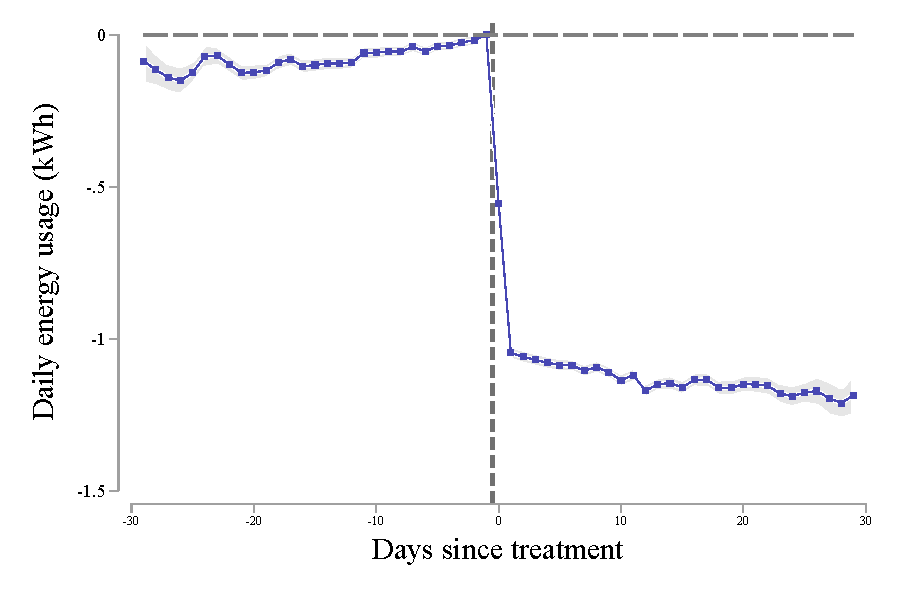
\includegraphics{HW6/event_study.pdf}{}
    \caption{Plot using coefplot.}
    \label{fig:enter-label}
\end{figure}

\item 
\begin{figure}[H]
    \centering
    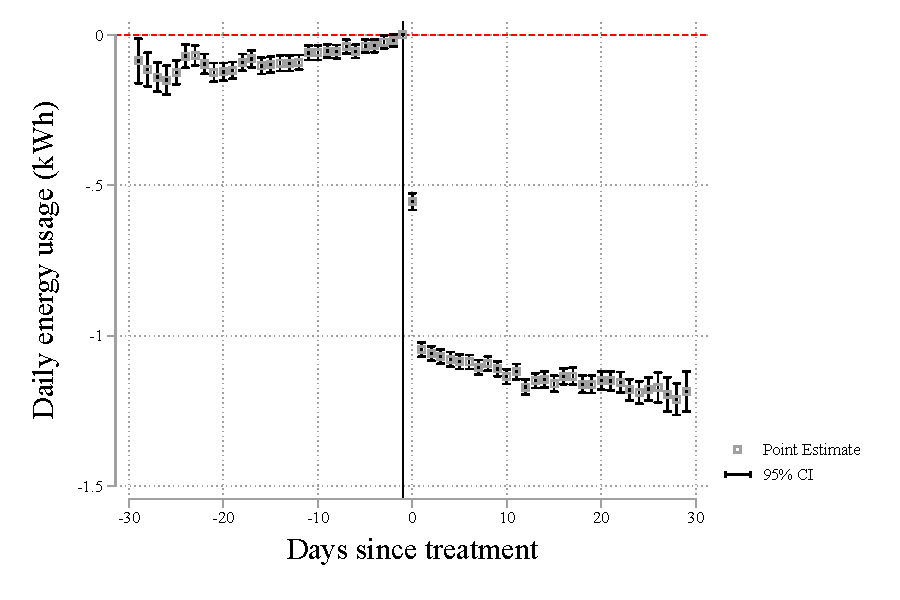
\includegraphics{HW6/eventdd_study.pdf}{}
    \caption{Plot using eventdd.}
    \label{fig:enter-label}
\end{figure}

\item 
\begin{figure}[H]
    \centering
    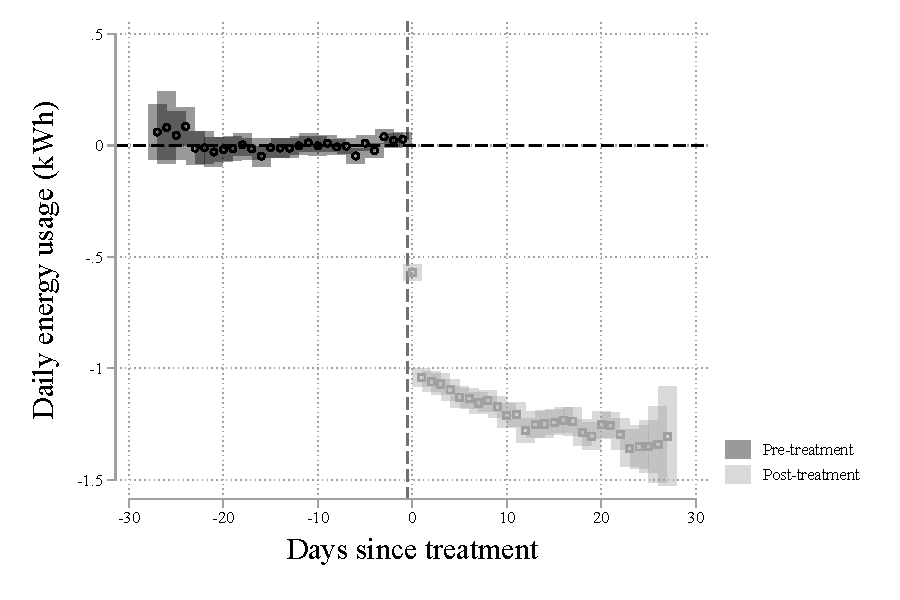
\includegraphics{HW6/event_study_csdid.pdf}{}
    \caption{CSDID package estimation.}
    \label{fig:enter-label}
\end{figure}



\end{enumerate} 
   
 \end{document}

